\chapter{Theoretical background}
    This chapter provides a necessary theoretical background. We start with a general overview of artificial intelligence areas, emphasizing the computer vision field and its approaches with follow-up tasks. Lastly, we try to address the metrics needed to evaluate the algorithms used in the thesis. A reader who is familiar with the thesis topic can continue straight to the next chapter.

\section{Relevant areas}
    In this section, we go through a brief explanation of topics such as artificial intelligence, machine learning, deep learning, and computer vision. The reason for this is that many people consider these terms as effectively synonymous, but it is not so.
    
    \subsection{Artificial intelligence}
        \Gls{ai} is an area of computer science that emphasizes the creation of intelligent machines that work and react like humans. The main characteristic is that, unlike traditional algorithms, the algorithms of artificial intelligence are capable of learning from new and past data. They can enhance themselves by learning new strategies, or they can themselves improve existing algorithms.
        
        Although creating a general artificial intelligence that is comparable to human has proved to be extremely difficult, over the past fifty years researchers have developed a set of procedures that achieve partial success in \gls{ai} sub-fields such as expert systems, genetic programming, state space search, data mining, machine learning, deep learning, and computer vision.
    
        \begin{figure}[ht]
            \centering
            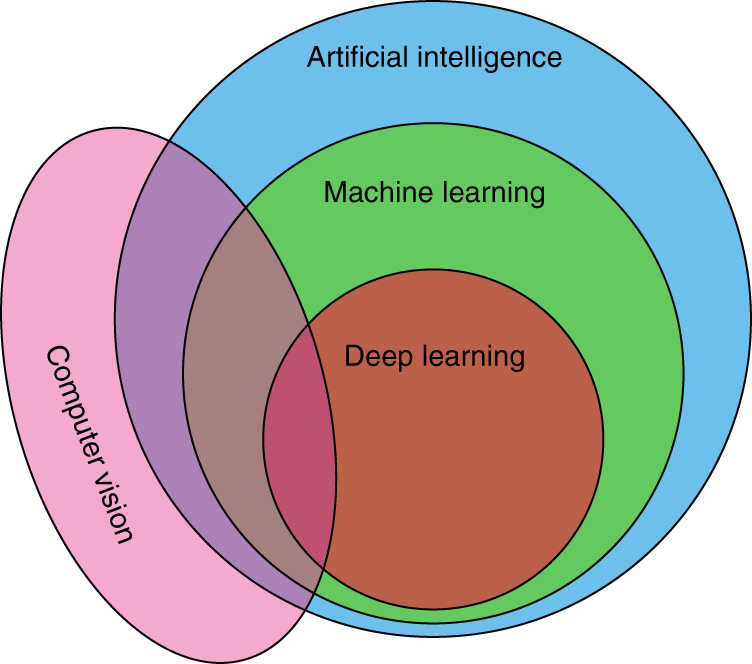
\includegraphics[width=0.75\textwidth]{resources/artificial_intelligence_set.png}
            \caption{Venn diagram of \gls{ai} and its sub-fields. Source: \cite{ruffle2018artificial}.}
            \label{fig:image_classification}
        \end{figure}
    
    \subsection{Machine learning}
        While \gls{ai} is a broader concept, \gls{ml} is the core part of it. It is focused on algorithms that can access data and learn from it automatically without human intervention. This is based on the assumption that we should give machines access to information and let them learn from it themselves.
        
        \Gls{ml} is sometimes considered difficult to understand. However, the basic intuition is not that complicated. At its core, we can imagine that \gls{ml} algorithm is just searching a decision hyperplane of best fit in many dimensions. If we have up to 2-D feature space of the problem, we can even visualize the hyperplane and the results. That is why dimensionality reduction such as \gls{pca} \cite{pearson1901liii} is often used. Moreover, the complexity in the machine learning tasks is the training and preparation of the training dataset. There is a great emphasis on the flawlessness of the dataset because if it contains errors, the algorithm can easily learn these imperfections and thus decrease the generalization performance. 
        
        There are three main \gls{ml} categories that are being actively researched. They differ from each other in the way they handle data, but also with the outputs they provide.
        
        \begin{figure}[h]
            \centering
            \subfloat[]{{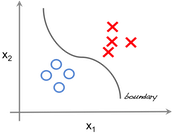
\includegraphics[width=3.8cm]{resources/supervised_learning.png} }}
            \qquad
            \subfloat[]{{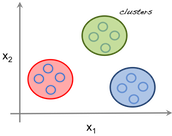
\includegraphics[width=3.8cm]{resources/unsupervised_learning.png} }}
            \qquad
            \subfloat[]{{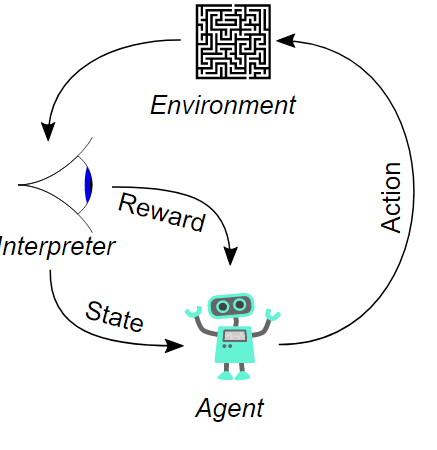
\includegraphics[width=3.4cm]{resources/reinforcement_learning.png} }}
            \caption{Categories of machine learning tasks. a) Supervised learning. b) Unsupervised learning. c) Reinforcement learning. Source: \cite{kuramasupervisedunsupervised, wiki:reinforcementlearning}}.
            \label{fig:ml categories}
        \end{figure}
        
        \subsubsection{Supervised learning}
            In supervised learning, the algorithm focuses on building a mathematical model from a set of available data that contains both the inputs and also the desired outputs. The most common example is to predict house prices based on various features such as the number of rooms, square floor feet, lot area, general condition, etc. \Gls{ml} model takes these features as inputs and based on its internal parameters, it produces output price prediction. This type of supervised learning is called regression. It is characterized by that the output is continuous value. Examples of continuous value are weight, length, temperature, price.
            
            Another type of supervised learning is classification which is used when the outputs are restricted to a limited set of values. We could consider a simple classification problem as identification of spam emails based on its words. The output prediction for this task would be of either "spam" or "not spam." A traditional supervised classification model used for decades is a \gls{svm} \cite{cortes1995support}, that divides the data into regions separated by a linear boundary. 
            
            There is also popular sub-category called semi-supervised learning that emphasizes on using incomplete data during training, in terms of missing labels for some data samples.
         
        \subsubsection{Unsupervised learning}
            Unsupervised learning algorithms try to build a mathematical model to find the patterns in data. The data given to the unsupervised model in training phase contains only input features and no desired output labels. Algorithms are then left to themselves to explore and discover critical structures in the data and group the inputs into categories. In the previous example with houses, the model would be able to find similar houses for input parameters, but not to predict the price of a given house. This process is known as clustering.
            
            Typical algorithm representatives for clustering are hierarchical clustering \cite{johnson1967hierarchical}, k-means \cite{macqueen1967some}, and DBSCAN \cite{ester1996density}.

            
        \subsubsection{Reinforcement learning}
            In the reinforcement learning, mathematical model, also called agent, is given feedback in the form of positive or negative reward in a dynamic environment. Given the agent's and environment's states, the agent takes actions which will maximize its reward or will explore a new possibility. These actions and rewards are then fed back into the agent and environment which will change their state. This step is repeated many times to improve the agent's behavior for future decisions. 
            
            Examples of rewards can be winning a game, scoring more points or earning more money. Thus it fits well dynamic tasks. Reinforcement learning, especially with deep neural network extension \cite{franccois2018introduction}, already performs well on a small human-involved task such as playing Atari games and it presents current state-of-the-art results in this field.
       
    \subsection{Deep learning}
        \Gls{dl} is a specialized form of \gls{ml} and it is currently the cutting edge of what machines can do - it has far surpassed any previous traditional algorithms for classification of images, text, and voice and we can find its use in all current machine learning applications. The essential advantage is that unlike \gls{ml} models, \Gls{dl} models are trained by large labeled sets of data where the model architecture learns the domain features directly without the need for manual feature extraction. This is also known as "end-to-end learning," where a model is given data, optimization criteria, and task to perform, and it learns how to perform this task automatically. Another important fact is that \gls{dl} models often continue to improve as the size of the data increases.
        
        \Gls{dl} tasks can be categorized into the same categories as \gls{ml} such as supervised, unsupervised, and reinforcement learning. The most common \gls{dl} models are based on an artificial neural network, which is why deep learning models are often referred to as deep neural networks. Unlike traditional neural networks with a few hidden layers, deep networks can have as many as a hundred. 
        
        Although many \gls{dl} approaches such as neural networks had been around for decades \cite{fukushima1980neocognitron, lecun1989backpropagation, lecun1998gradient}, some researches asses that victory of Krizhevsky in October 2012 ImageNet competition started the "deep learning revolution" \cite{russakovsky2015imagenet}. However, it was not the only big break. Google’s Deep reinforcement learning based AlphaGo beating the best Go player in the world \cite{kochgo} also had a great impact on the research community. 
        
        There are two main drawbacks while using \gls{dl} approaches. Firstly, it requires a large amount of labeled data. In an example such as autonomous driving, it is often required to have thousands of hours of video, which can take up a few petabytes of storage space. Secondly, \gls{dl} requires substantial computing power, which is most often achieved by using high-performance \gls{gpu}s that have parallel architecture. However, most people, including researchers, do not have their \gls{gpu} cluster, so they use cloud computing that enables them to reduce training time from weeks to hours. There are also many criticism concerns around \gls{dl} because methods are often looked at as a block box with the lack of theory, with most confirmations done empirically rather than theoretically.
        
    \subsection{Computer vision}
        \Gls{cv} is the process of using machines to process, understand and analyze various types of image data in order to produce numerical or symbolic information, e.g., in the forms of decisions. The motivation is to automate tasks that human visual systems can do to utilize human resources on more critical tasks. Moreover, with a large number of surveillance cameras, it is not possible to monitor all of them by people. 
        
        \begin{figure}[ht]
            \centering
            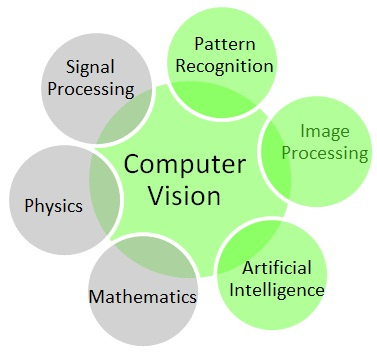
\includegraphics[width=0.55\textwidth]{resources/computer-vision-venn.png}
            \caption{Venn diagram of related fields of \gls{cv}. Source: \cite{khandelwalcv}}.
            \label{fig:convolutional neural netwok}
        \end{figure}
        
        The whole process of deciding over imagery data is called a \gls{cv} pipeline. The traditional pipeline starts with image acquisition, followed by image preprocessing and feature extraction step, ending with a classifier. This pipeline follows well-established principles from any machine learning task. Therefore, we do not consider it necessary to explain it in this work. However, a detailed description of each step can be found in \cite{koenpieline}.
    
        The analyzed image data can be a standard photo or video sequence from a single RGB camera, but also to more complex data such as multiple camera video sequence and multi-dimensional imagery from satellite or medical equipment. Machines interpret this visual content very straightforwardly - as a series of pixels that forms a grid (matrix), where each pixel has its own set of color values (see Fig. \ref{fig:lincon_pixels}). However, in order for the machines to make decisions, they need to understand higher-level concepts in the data, not to use just plain pixel values. Since the size of the imagery data is large, feature extraction is a common technique to obtain high-level features thus helping machines to understand the visual context. 
        
        \begin{figure}[h]
            \centering
            \subfloat[]{{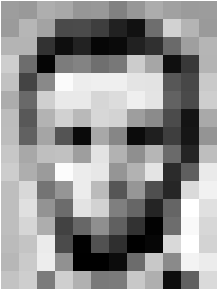
\includegraphics[width=3.5cm]{resources/lincoln_pixel_values_1.png} }}
            \qquad
            \subfloat[]{{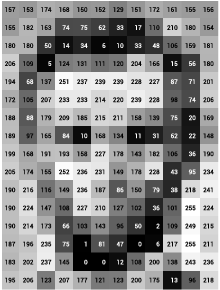
\includegraphics[width=3.5cm]{resources/lincoln_pixel_values_2.png} }}
            \qquad
            \subfloat[]{{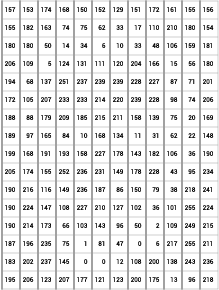
\includegraphics[width=3.5cm]{resources/lincoln_pixel_values_3.png} }}
            \caption{Pixel data diagram of simplified grayscale image. a) The image itself. b) The pixels labeled with numbers from 0-255, representing their brightness. c) Pixel numbers by themselves. Source: \cite{computervisiongolan}}.
            \label{fig:lincon_pixels}
        \end{figure}
        
        To this date, we can observe two main approaches in \gls{cv} pipelines - hand-crafted \gls{ml} methods and \gls{dl} methods. The main difference is how features are obtained before the algorithm decision is made. We can think of mean, variance, median, min, and max of our data as useful measures for discrimination of samples. Since these features are specified explicitly, they are called hand-crafted. In practice, we have more complicated tasks that require more sophisticated statistical functions and complex feature extractors such as Haar \cite{viola2001rapid}, LBP \cite{ojala2002multiresolution}, HoG \cite{dalal2005histograms}, SIFT \cite{lowe2004method}, SURF \cite{bay2006surf}, but the idea is the same - we know how the features will look like in advance. In \gls{dl}, we know nothing about the features until we learn them from data itself. We still need to specify model and its parameters, but the real feature learning is achieved by an iterative optimization process.
        
         \Gls{cv} is nowadays ubiquitous in our society. It is used in applications such as image understanding, medicine, self-driving cars, augmented reality, and drones and there are many sub-domains of \gls{cv} that are actively researched. The most significant interest is currently on scene reconstruction, object detection and tracking, human pose estimation, and style transfer. It may be a surprise, but the core of many applications often builds upon something simple as image classification, and while many types of \gls{cv} algorithms have been around since the 1960s, recent developments in computing capabilities have driven significant improvements in how well machines understand the image content. Furthermore, with the advent of \gls{dl} approaches, \gls{cv} is becoming increasingly popular, and at the same time, there is a noticeable increase in the accuracy of many existing \gls{cv} applications. 
     
\section{Computer vision approaches}
    Because the computer vision field has massively transformed into \gls{dl} algorithms, we present a brief overview of some conventional approaches that are used for solving computer vision tasks.
    
    \subsection{Artificial neural network}
        \Gls{ann}, or simply \gls{nn} in this context, is an interconnected graph of artificial neurons that uses computational model for solving \gls{ml} tasks. In more practical terms, \gls{nn} are non-linear statistical data modeling or decision making tools that can be used to model complex relationships between inputs and outputs or to find patterns in data. In most cases, a \gls{nn} adapts its internal structure based on information that flows through the network. Thanks to many breakthrough results in recent years, it generated much excitement in the research community. 
        
        \subsubsection{Artificial neuron}
            There are many types of \gls{nn}s. However, the most researched and utilized is a particular type known as the \gls{mlp}. Its basic unit of computation is called neuron (or node). It receives input from other neurons and computes an output value. Each input $x_i$ of a neuron has its a particular weight $w_i$ value associated. The weight can be understood as relative importance to other neuron inputs. Weights and inputs are added together in weighted sum and additional bias term $b$ is used to correct this value. In the end, activation function $\varphi$ is used to generate an output of the neuron $y_k$.  In mathematical notation, the output of a neuron is given by:
    
            \begin{equation}
                y_k = \varphi \left(\sum\limits_{j=1}^n w_j x_j + b \right)
            \end{equation}
        
        \subsubsection{Activation function}
            Since most of the real world data are non-linear, the activation function must be non-linear too. This is also very important for Universal approximation theorem \cite{hornik1989multilayer}, which says that a \gls{mlp} can approximate any function, i.e., can in principle learn anything. To this date, many activation functions were proposed, but the most commonly known are:
            
           \begin{itemize}
                \item \textbf{Sigmoid} - The sigmoid non-linearity squashes real numbers to range between $[0,1]$.
                
                \begin{equation}
                   \sigma(x) = \frac{1}{1 + e^{-x}}
                \end{equation}
                
                \item \textbf{tanh} - The tanh non-linearity squashes real numbers to range between $[-1,1]$.
                
                \begin{equation}
                    \tanh(x) =  2\sigma(2x) - 1
                \end{equation}
                
                \item \textbf{ReLU} - The activation value of ReLU is simply thresholded at zero. As the ReLU has proved to work very well, several other variants such as Leaky ReLU, ELU, and SELU have emerged.
                
                \begin{equation}
                    f(x) = \max(0, x)
                \end{equation}
            \end{itemize}
    
            The activation function selection is crucial for task accuracy and performance. However, their thorough description is very comprehensive. Hence we recommend \cite{cs231n} for their detailed overview.

        \subsubsection{Feed-forward neural network}
            Feed-forward \gls{nn} contains multiple neurons arranged in layers. Nodes from adjacent layers have connections between them, and all these connections have associated weights. In this type of network, the information moves only in the forward direction, hence the name. No cycles are allowed in this network architecture.
            
            A feed-forward neural network can consist of three types of layers:
            
            \begin{itemize}
                \item \textbf{Input layer} - The input layer is always at the beginning of the network. It provides information from outside of the model to the network. No computation is performed at this stage; values are just passed to further neurons.
                \item \textbf{Hidden layer} - Neurons in this layer perform computations to output nodes based on input nodes and internal parameters. A feed-forward network can have zero or multiple hidden layers.
                \item \textbf{Output layer} - This layer is responsible for transferring the computed information from the network to the outside world. The transferred information usually represent a class probability score or some real-valued prediction.
            \end{itemize}
           
            The weights in neurons are iteratively improved in the training phase, where data is forwarded through the network,  then the difference between ground-truth and the predicted value is calculated. The procedure to improve the weights is known as backpropagation \cite{hecht1992theory}.  An example of a feed-forward neural network is shown in Fig. \ref{fig:neuron and neural network}. Feed-forward \gls{nn} with many hidden layers is called deep \gls{nn}.

            \begin{figure}[ht]
                \centering
                \subfloat[]{{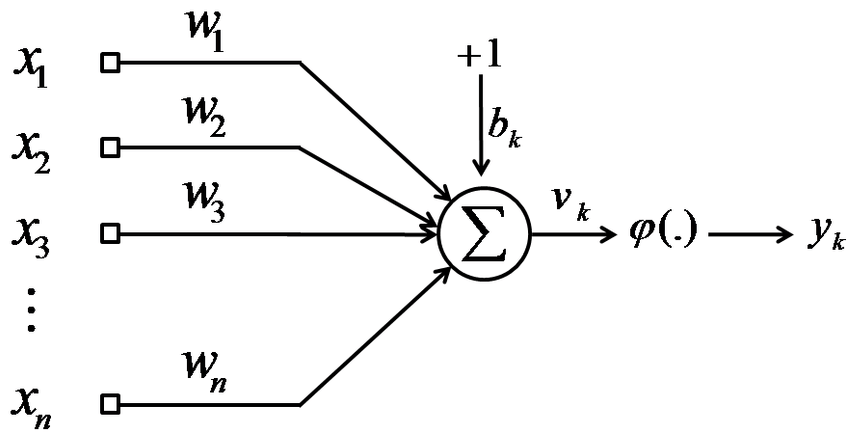
\includegraphics[width=0.35\textwidth]{resources/single_neuron.png} }}
                \qquad
                \subfloat[]{{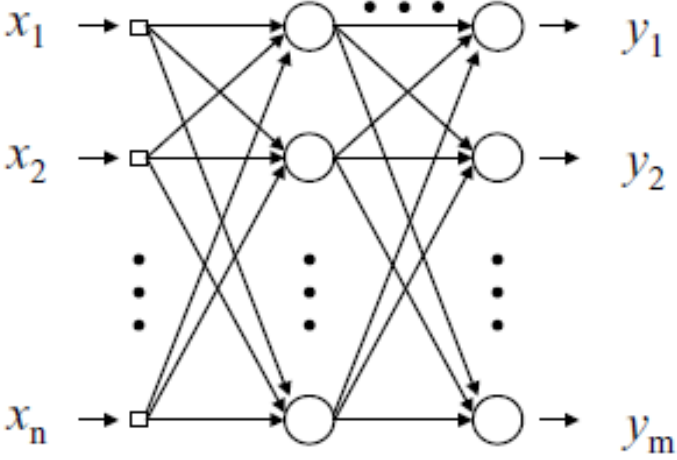
\includegraphics[width=0.35\textwidth]{resources/neural_network.png} }}
                \caption{Pixel data diagram of simplified grayscale image. a) Schematic of a single neuron. b) Schematic of a feed-forward neural network. Source: \cite{nnfurtado}}.
                \label{fig:neuron and neural network}
            \end{figure}
            
    \subsection{Convolutional neural network}
        One of the most common methods for solving computer vision task is \gls{cnn}. It uses convolutional layers to learn features from input data without minimal preprocessing. Hence it eliminates the need for manual feature extraction as in traditional methods. The features are learned while the \gls{cnn} trains on large labeled image dataset. This approach has shown to be highly accurate since it outperforms humans in image recognition task \cite{russakovsky2015imagenet} and it is is one of the most popular techniques for deep learning. Current applications such as object self-driving cars, object detection, medical image classification, combined with advances in GPUs and parallel computing, heavily relies on \gls{cnn} architectures. 

        A \gls{cnn} can have tens to hundreds of layers that each learn to detect different patterns or features of an image. Depth of the \gls{cnn} is critical component for a good performance \cite{russakovsky2015imagenet}. Since there is the explicit assumption that the inputs are grid-like topology, such as an image, certain properties are encoded into layer architecture that makes the forward function more efficient by reducing the number of parameters in the network. Network layers perform operations that alter the data with the intent of learning features specific to the data. Three of the most important layers are convolution, activation, and pooling which are often applied multiple times in a row before concluding the process of feature extraction. The goal of repetition is to identify different features, and the argument for this is the observation that images contain hierarchical structure (e.g., faces are made up of eyes, which are made up of edges, etc.), so several layers of processing will increase in extracted features complexity to features that uniquely define particular object. The outputs of this whole process are then often passed into a fully connected layer for final output, i.e., class score probabilities. 
        
        Layout, number, and type of layers form the architecture of the \gls{cnn}. To this date, dozens of architectures were proposed, and the most famous are LeNet, AlexNet, VGGNet, Inception, ResNet, ResNeXt, and DenseNet. Since each of these architectures would require extensive description, we consider it as out of the scope of this thesis, and we suggest \cite{cs231n, dascnnoverview, jordancnnoverview} for further reading. 

        \begin{figure}[ht]
            \centering
            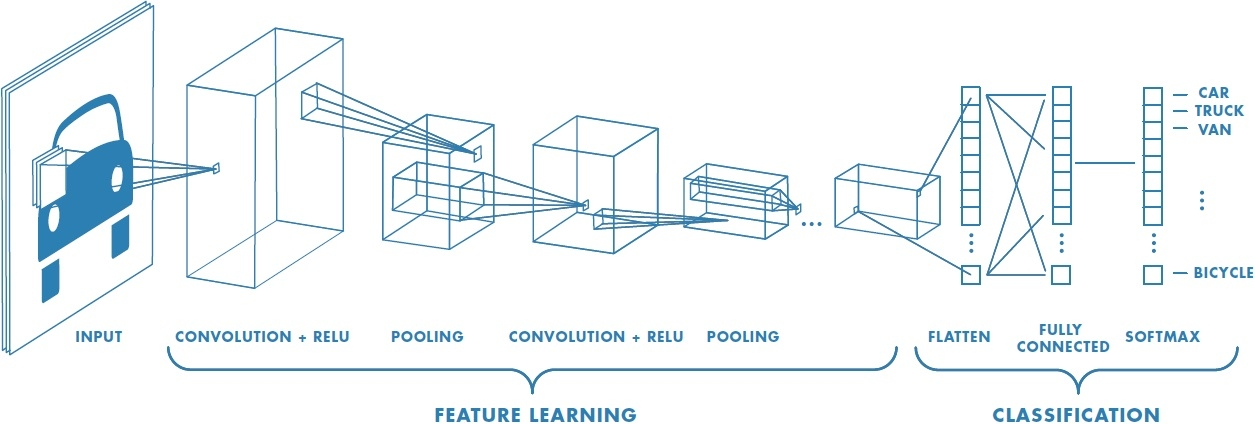
\includegraphics[width=0.85\textwidth]{resources/convolutional-neural-network.png}
            \caption{Example of a network with many convolutional layers. Filters are applied to each training image at different resolutions, and the output of each convolved image is used as the input to the next layer. Source: \cite{mathworkscnn}}.
            \label{fig:convolutional neural netwok}
        \end{figure}
        
        \subsubsection{Convolution layer}
            The convolution layer is the core building block of any \gls{cnn}, where the input image pixels are modified by a convolutional filter, which is a matrix that is multiplied with different parts of the input image. The filter is spatially smaller than an image (e.g., 3x3, 5x5, 8x8), but is more in-depth. Each filter aims to activate certain features from the images. The output this layer is known as feature map (alternatively activation map) which is usually smaller in size but has more dimensions. Ideally, a feature map will be less redundant and more informative than the original input.
            
        \subsubsection{Activation layer}
            The purpose of this layer is the same as in the \gls{ann}, to introduce non-linearity in the feature map. Favorite choice in the \gls{cnn} case is ReLU due to its simplicity, hence effective training process.
            
        \subsubsection{Pooling layer}
            Since the convolutional layer expands dimensionality, pooling is a process that reduces the size of the feature map by a factor of whatever size is pooled. The consequence is the reduction of the number of parameters that the network needs to learn. The input image is scanned over each dimension by a sliding window and either the max, sum or average the window is taken as a representation of that portion of the image. 
            
        \subsubsection{Fully-connected layer}
            A fully-connected layer is most often the last layer of the \gls{cnn} architecture. It stands for common feed-forward \gls{nn} with fixed input size explained in the previous section. Adding this type of layer usually helps with combining the high-level features from convolutional layers into a non-linear function. The fully connected network outputs a vector that contains the probabilities of each object class of an image being classified.


    \subsection{Transfer Learning}
        It is sporadic for people to train an entire \gls{cnn} from scratch. There are three main reasons for this. Firstly, it has been proved that \gls{cnn} and \gls{nn} are very sensitive to proper weights initialization. Many works have been done on this topic, and it is generally not recommended to use random or zero initialization since it can lead to the vanishing or exploding gradients. Secondly, there are very few datasets with sufficient size. Using only a tiny dataset will lead to insufficient accuracy and overfitting. Lastly, the training phase is computationally intensive. Modern \gls{cnn} architectures can take a few weeks to train on multiple \gls{gpu}s properly.

        In practice, it is common to take pretrained parameters from existing \gls{cnn} used for similar task (e.g., ImageNet classification \cite{russakovsky2015imagenet}, which contains 1.2 million images with 1000 categories) and use them as initialization or a fixed feature extractor for the task of interest. It is very straight-forward to use existing \gls{cnn} as a feature extractor, only the last fully-connected layer needs to be removed or replaced.
        
\section{Computer vision tasks}
    In this section, we provide a quick overview of tasks relevant to the thesis topic and their specific challenges. Since the first early steps of computer vision field in the 1960s, the scientists tried to build camera robots with intelligent behavior. However, it turned out to be a much more complex problem than they initially thought and as a first step, they desire was to extract three-dimensional structure from two-dimensional images to achieve full scene understanding, thus forming the very first computer vision task - scene reconstruction. This time was the foundation for many computer vision algorithms that exist today, including edge detector and lines extractors. Later, the robots, who now understood the scene, needed to move around while avoiding obstacles. This could be accomplished through motion analysis. Some existing algorithms such as Kalman filter already existed. Therefore, they were adapted to \gls{cv} field. Recent work is mostly focused on feature-based methods used together with machine learning algorithms to produce numerical or symbolic information for decision making. 
    
    \begin{figure}[ht]
        \centering
        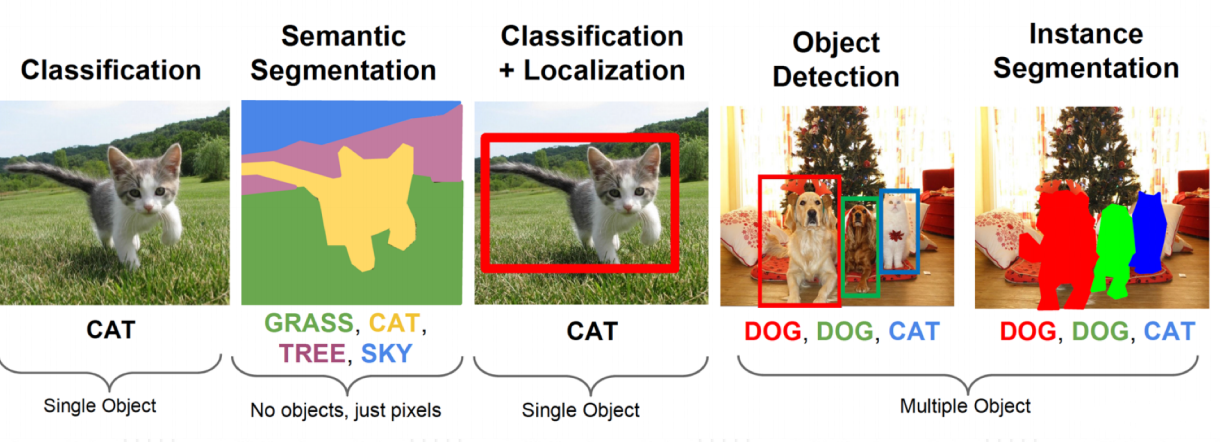
\includegraphics[width=0.95\textwidth]{resources/computer-vision-tasks.png}
        \caption{Common computer vision tasks. Source: \cite{cs231n}.}
        \label{fig:computer-vision-tasks}
    \end{figure}
    
    \subsection{Image classification}
        The typical problem in computer vision field is that of determining if image data contain a specific object. Image classification, with its main component known as classifier, is a particular application of computer vision which assigns an input image one label from a fixed set of categories. The general approach is to assign probabilities for each class and then choose the most likely one. Despite its simplicity, it is one of the core problems in computer vision with a large variety of applications. Moreover, many other distinct computer vision tasks (localization, object detection, segmentation, etc.) can be reduced to image classification.
        
        In Fig. \ref{fig:image_classification}, we can see the image of a cat with associated probabilities of belonging into four categories. We need to keep in mind that in this case, the image is represented as a large 3-dimensional matrix of numbers in a machine's memory. In this figure, the image is 248 pixels wide, 400 pixels tall, and has three color channels. Therefore, the image consists of 248 x 400 x 3 numbers, or a total of 297,600 numbers. Each number is an integer that ranges from 0 (black) to 255 (white). The task is to turn a quarter of a million numbers into a single label, such as “cat.” \cite{cs231n}
        
        \begin{figure}[ht]
            \centering
            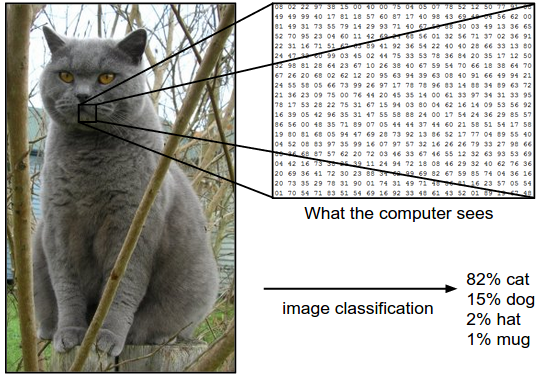
\includegraphics[width=0.75\textwidth]{resources/image_classification.png}
            \caption{Image classification example. Source: \cite{cs231n}.}
            \label{fig:image_classification}
        \end{figure}
    
        Since this task of recognizing objects is relatively trivial for humans, it only makes sense to consider challenges for \gls{cv} algorithms. The challenges are shown in Fig. \ref{fig:image_classification_challenges} and they are especially:
    
        \begin{itemize}
            \item \textbf{Viewpoint variation} - A single instance of an object can be oriented in many ways concerning the camera.
            \item \textbf{Scale variation} - Visual classes often exhibit variation in their size (size in the real world, not only in terms of their extent in the image).
            \item \textbf{Deformation} - Many objects of interest are not rigid bodies and can be deformed in extreme ways.
            \item \textbf{Occlusion} - The objects of interest can be occluded. Sometimes only a small portion of an object could be visible.
            \item \textbf{Illumination conditions} - The effects of illumination are drastic on the pixel level.
            \item \textbf{Background clutter} - The objects of interest may blend into their environment, making them hard to identify.
            \item \textbf{Intra-class variation} - The classes of interest can often be relatively broad, such as a chair. There are many different types of these objects, each with their appearance.
        \end{itemize}
        
        \begin{figure}[ht]
            \centering
            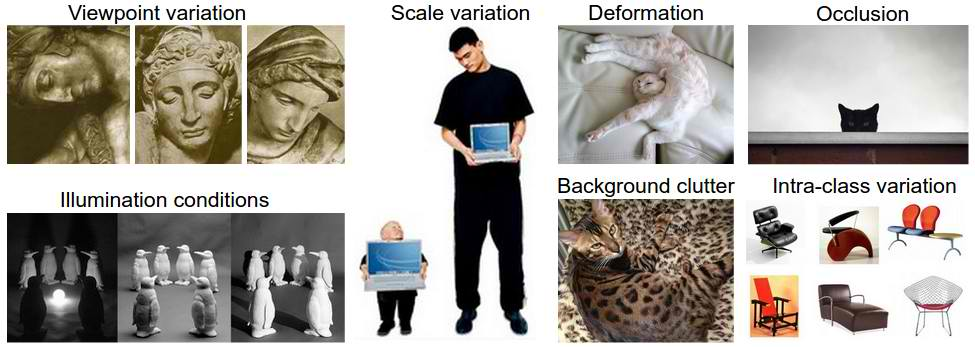
\includegraphics[width=0.85\textwidth]{resources/image_classification_challenges.png}
            \caption{Image classification challenges. Source: \cite{cs231n}.}
            \label{fig:image_classification_challenges}
        \end{figure}
        
         A good image classification model must be invariant to the cross product of all these variations, while simultaneously retaining sensitivity to the inter-class variations. \cite{cs231n}
         
    \subsection{Object detection}
        Image classification models can classify input images into the most likely category. However, typical images including photos are usually more complex and contain multiple objects. Therefore, assigning single object category does not make much sense. Object detection is a well-researched and more appropriate method that helps to identify multiple objects from predefined categories from a single image. The output of the typical object detector is an object's bounding box, category, and confidence of the detection. The coordinates of the bounding boxes can be then used for further visual tasks.
        
        The first important object detector based on Haar cascades was proposed by Paul Viola and Michael Jones in 2001 \cite{viola2001rapid}. It was able to operate in real-time and was subsequently implemented in digital cameras. Although it could be trained to detect a variety of object classes, it was used mainly for the face detection task. After a long time, in 2005, another promising detector known as \gls{hog} \cite{dalal2005histograms} was introduced. It was focused for pedestrian detection in static images and was further improved for video sequences, as well as to a variety of object classes including animals and vehicles. \Gls{hog} has been used for a long time in conjunction with other feature extractors for various detection tasks until the success of \gls{dl} architecture in 2012 ImageNet competition \cite{russakovsky2015imagenet}. Since then, the use of conventional detectors is mostly replaced with deep neural networks.
        
        In object detection based on \gls{cnn}s, there are two main core design choices. First is, hypothesize object regions and then classify them. Second, divide the image into a grid and directly predict bounding boxes and class probabilities in a single evaluation - only one feed-forward pass. A few state-of-the-art representatives for each category are briefly reviewed below. For their detailed overview, we suggest \cite{huang2017speed, xuobjectdetection, ouaknineobjectdetection}.
        
        \subsubsection{\Glsentryfull{r-cnn}}
            \Gls{r-cnn} \cite{girshick2016region} is very first and intuitive architecture that started the era of object detection with \gls{cnn}s. The pipeline of the model begins with scanning the input image for possible objects using Selective Search algorithm \cite{uijlings2013selective}. This method generates a large number of proposals that are reduced to some reasonable amount (typically to order of thousands). Moreover, each proposal is also resized to match the input of a \gls{cnn}, which is used to extract image features. The output vector of the \gls{cnn} is fed into a \gls{svm} classifier to verify if an object exists within the region and if yes, a linear regressor is used to refine the bounding box.
            
            \begin{figure}[ht]
                \centering
                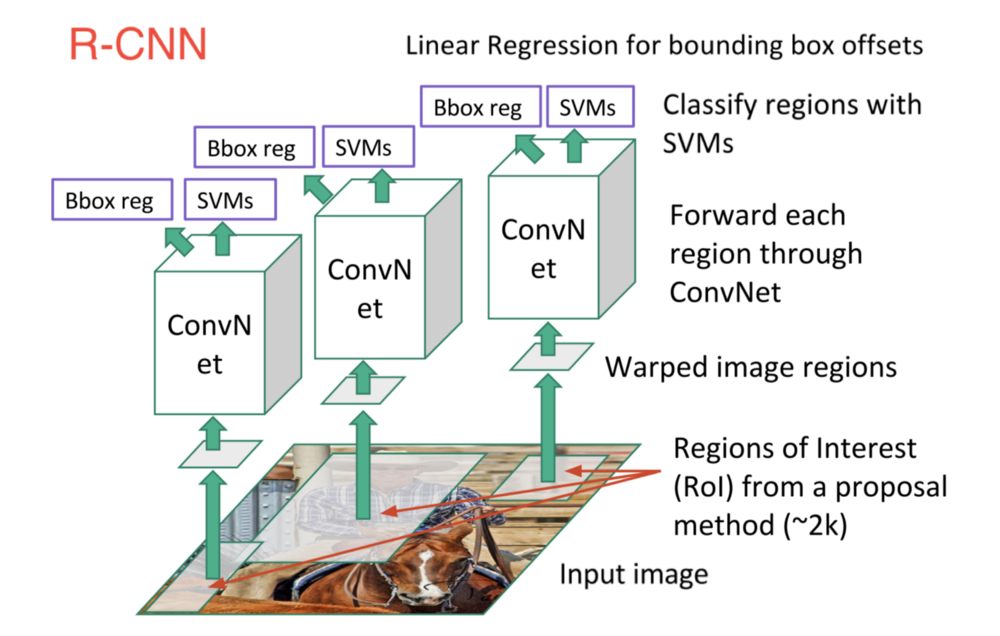
\includegraphics[width=0.85\textwidth]{resources/r_cnn_architecture.png}
                \caption{\Gls{r-cnn} architecture. Source: \cite{xuobjectdetection}.}
                \label{fig:r-cnn architecture}
            \end{figure}
        
            To sum it up, this approach turns object detection into an image classification discussed before. The drawback of this method is that the training and inference are very slow. For example, the inference time for a single image varies from tens of seconds to minutes.

        \subsubsection{\Glsentryfull{fast r-cnn}}
            Just year after the publication of \gls{r-cnn}, the same authors improved the approach with new \gls{fast r-cnn} \cite{girshick2015fast} architecture. It resembled the original in many ways. However, they drastically improved the training and testing speed performance.
            
            The improvement consisted of two main aspects. The feature extraction run by \gls{cnn} is no longer run thousands time over proposed regions, but only once over the entire image. The regions are still obtained by Selective search algorithm. However, its input is the output of the \gls{cnn} - feature map. The proposed regions are then reshaped using an RoI pooling layer and instead of training many different \gls{svm} classifiers for each object class, there is a single fully connected \gls{nn} with softmax layer that outputs the class probabilities directly.
            
            \begin{figure}[ht]
                \centering
                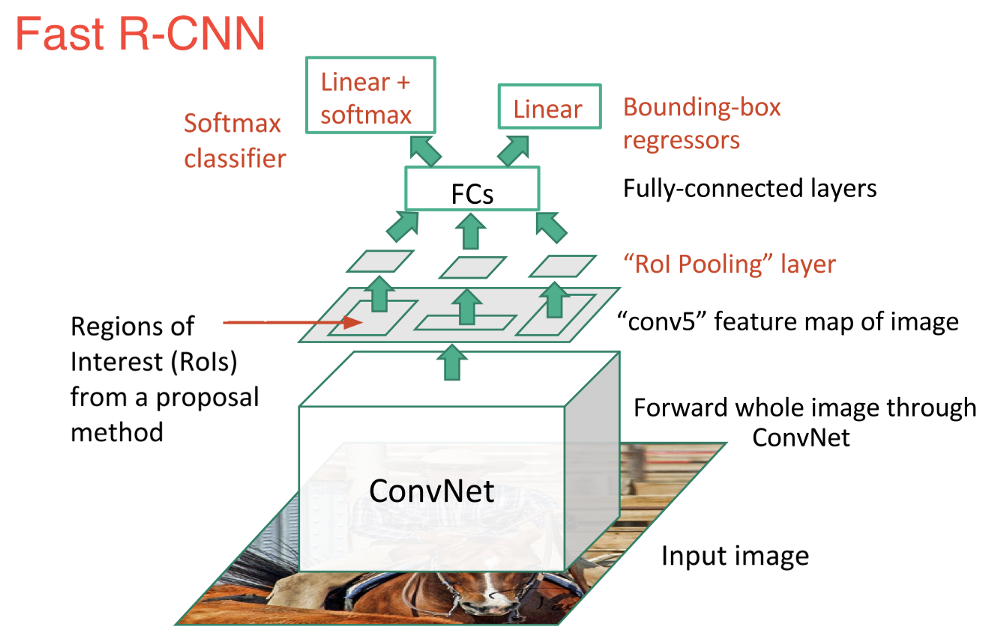
\includegraphics[width=0.85\textwidth]{resources/fast_r_cnn_architecture.png}
                \caption{\Gls{fast r-cnn} architecture. Source: \cite{xuobjectdetection}.}
                \label{fig:fast r-cnn architecture}
            \end{figure}
    
        \subsubsection{\Glsentryfull{faster r-cnn}}
            Both of the architectures mentioned above use a Selective Search algorithm to find out the region proposals. However, it turned out that Selective Search is the computational bottleneck. Besides that, it has another big disadvantage - it is a fixed algorithm; no learning is happening which can lead to bad region proposal candidates. Therefore, a new architecture know as \gls{faster r-cnn} \cite{ren2015faster} was introduced to improve these shortcomings. 
            
            \Gls{faster r-cnn} completely replaced the use of the Selective Search algorithm with a separate \gls{nn} (known as the \gls{rpn}) to identify region proposals. The \gls{rpn} is run right after the feature extraction, and once we obtain the region proposals, they are feed into what is essentially \gls{fast r-cnn}.

            \begin{figure}[ht]
                \centering
                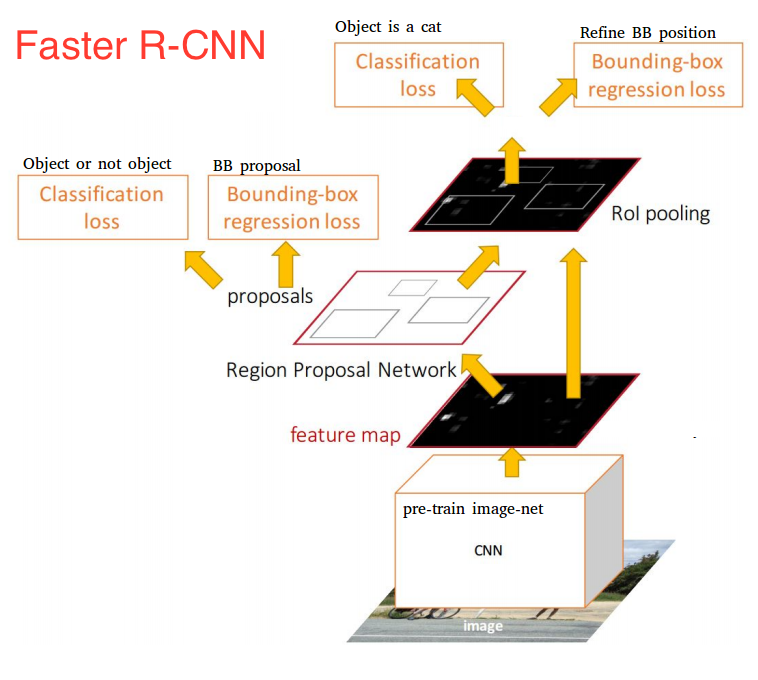
\includegraphics[width=0.85\textwidth]{resources/faster_r_cnn_architecture.png}
                \caption{\Gls{faster r-cnn} architecture. Source: \cite{xuobjectdetection}.}
                \label{fig:faster r-cnn architecture}
            \end{figure}
            
            To be concise, \gls{faster r-cnn} is combination between the \gls{rpn} and \gls{fast r-cnn}. It is much faster than its predecessors, and it can even be used for real-time object detection in a video sequence. To date, it is still widely used thanks to its speed and accuracy performance.
            
        \subsubsection{\Glsentryfull{yolo}}
            All of the previous object detection algorithms use proposed regions to localize the object within the image. It means that the detector does not look at the whole image. Instead, it evaluates regions which have high probabilities of containing the object. In \gls{yolo} \cite{redmon2016you}, a single \gls{cnn} directly predicts bounding boxes and class probabilities with a single forward pass.
            
            Initially, the model takes the input image and divides it into an SxS grid. Within each cell of the grid, m bounding boxes are taken. For each of selected bounding box, the network outputs a class probability and refinement for the bounding box. If bounding box has the class probability above a threshold value, it is then used to locate the object within the image. Since the model predicts a high number of bounding boxes, the \gls{nms} method is applied at the end of the network to merge highly-overlapping bounding boxes of the same object into a single one.
            
             \begin{figure}[ht]
                \centering
                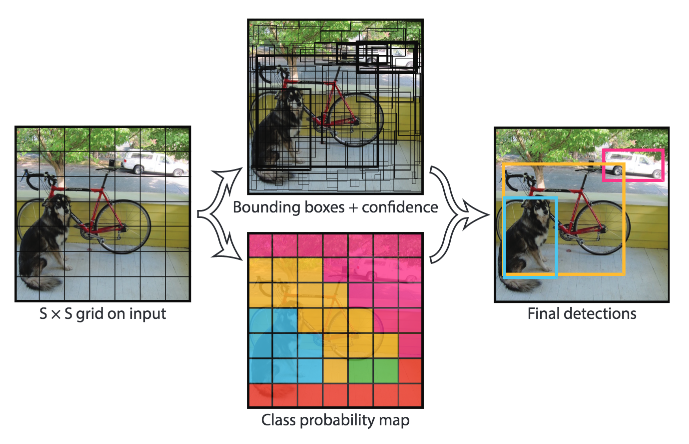
\includegraphics[width=0.85\textwidth]{resources/yolo_approach.png}
                \caption{Example of \gls{yolo} approach. Source: \cite{redmon2016you}.}
                \label{fig:yolo approach}
            \end{figure}
            
            Due to its simplicity, it is much faster than other detection algorithms mentioned. Depending on the backbone architecture, it can run approximately 15 to 150 \gls{fps}. The limitations of \gls{yolo} are that it struggles with small objects and unusual aspect ratios, which is due to the spatial constraints of the algorithm.

    % \subsection{Instance segmentation}

    \subsection{Face recognition}
        Face recognition is a prominent biometric technique that is used for everything from automatically tagging pictures on social networks to unlocking cell phones. It has been a long-standing research topic in the \gls{cv} community since it uses \gls{cv} algorithms to extract specific and distinctive information about a person's face, such as distance between the eyes, shape of the chin. This information is then converted to a feature vector and stored into a face database. It is desired only to include specific details that can distinguish one face from another to maintain a reasonable size of the feature vector. 
        
        Each facial feature vector can be compared to others to find the most likely match which helps to verify personal identity. However, some face recognition systems are designed to calculate a probability match score to provide several potential matches, instead of just returning a single result. The results of face recognition systems can vary under challenging conditions such as poor lighting, low resolution, improper angle of view.
        
        For decades, only traditional methods such as filtering responses, a histogram of the feature codes, or distribution of the dictionary atoms were used to recognize faces. However, these approaches were improving the accuracy very slowly and were suffering from a lack of distinctiveness and compactness. Effects of lighting, pose and expression drastically worsened the results. Fortunately, this has all changed with the advent of \gls{dl}. In 2014, DeepFace \cite{taigman2014deepface} approach achieved the state-of-the-art accuracy on the famous face recognition benchmark, approaching human performance on the unconstrained condition for the first time. This has caused this field to move in the direction of \gls{dl}, and it completely reshaped all aspects of face recognition. On Fig. \ref{fig:deep face recognition} the typical pipeline of face recognition is visualized.
        
        \begin{figure}[ht]
            \centering
            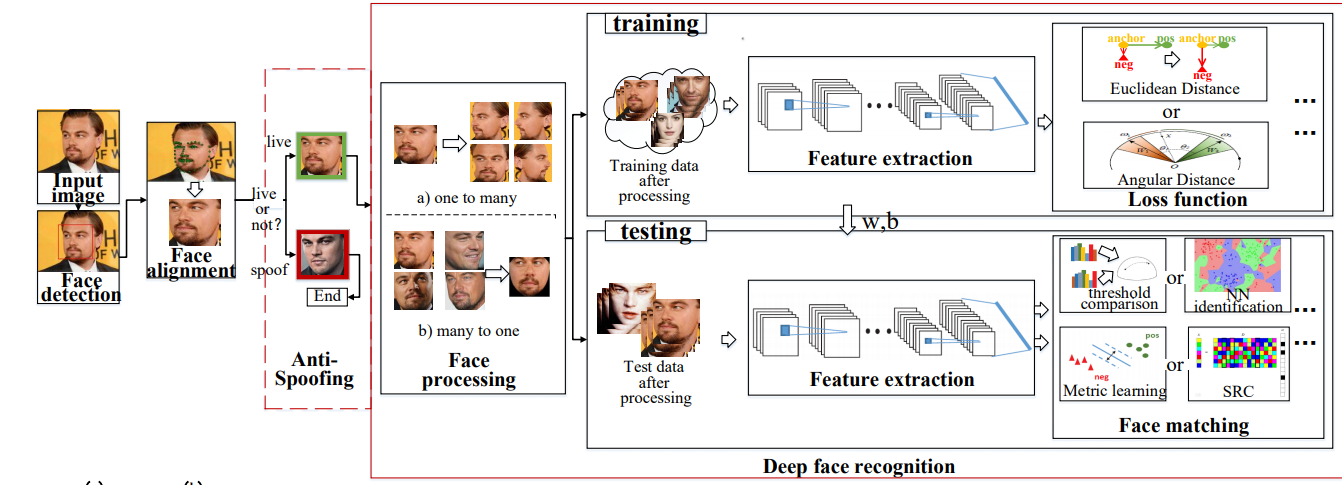
\includegraphics[width=1\textwidth]{resources/deep_face_recognition.png}
            \caption{Common pipeline for state-of-the-art face recognition systems. Source: \cite{wang2018deep}.}
            \label{fig:deep face recognition}
        \end{figure}

    \subsection{Motion analysis}
     
    \subsection{Scene reconstruction}

\section{Software frameworks}
    Research in the fields of artificial intelligence requires the use of analytical tools, technologies, and languages to help extract insights and value from data, and after that build sustainable mathematical model.
    The key advantages of using frameworks and libraries are the ability to quickly develop and test new ideas and run efficiently on \gls{gpu}.

    According to a 2017 survey of 16,000 data scientists by Kaggle revealed that scientists most rely on Python language \cite{mostuseddatasciencetools}. So there is no surprise that most of these packages are developed for that language. For this reason, we provide a quick overview of significant and common Python \gls{ml} frameworks.
    
    \subsection{TensorFlow}
        TensorFlow is an open source software library for numerical computation using data flow graphs. The graph nodes represent mathematical operations, while the graph edges represent the multidimensional data arrays (tensors) that flow between them. This flexible architecture enables users to deploy computation to one or more CPUs or GPUs in a desktop, server, or mobile device without rewriting code. TensorFlow also includes TensorBoard, a data visualization toolkit.

        TensorFlow was originally developed by researchers and engineers working on the Google Brain team within Google's Machine Intelligence Research organization for the purposes of conducting machine learning and deep neural networks research. The system is general enough to be applicable in a wide variety of other domains, as well.

        TensorFlow provides stable Python and C APIs as well as non-guaranteed backwards compatible API's for C++, Go, Java, JavaScript, and Swift. \cite{abadi2016tensorflow}
        
    \subsection{PyTorch}
        PyTorch is an open source library designed to enable rapid research on machine learning models. It builds upon a few projects, most notably Lua Torch, Chainer, and HIPS Autograd, and provides a high-performance environment with easy access to automatic differentiation of models executed on different devices (CPU and GPU). To make prototyping easier, PyTorch does not follow the symbolic approach used in many other deep learning frameworks, but focuses on differentiation of purely imperative programs, with a focus on extensibility and low overhead. \cite{paszke2017automatic}
        
    \subsection{Caffe2}
        Caffe2 aims to provide an easy and straightforward way for users to experiment with deep learning and leverage community contributions of new models and algorithms. Users can bring their creations to scale using the power of GPUs in the cloud or to the masses on mobile with Caffe2's cross-platform libraries. In May 2018, the development team decided to merge Caffe2 into PyTorch and make them a single package to enable a smooth transition from fast prototyping to fast execution. \cite{caffe2}
        
    \subsection{Theano}
        Theano is a Python library that allows to define, optimize, and evaluate mathematical expressions involving multi-dimensional arrays efficiently. Since its introduction in 2008, it has been one of the most used CPU and GPU mathematical compilers – especially in the machine learning community - and has shown steady performance improvements. However, the development team decided to stop further releases in 2017. \cite{2016arXiv160502688short}
        
\section{Evaluation metrics}
    In this section, we provide a brief overview of common evaluation metrics relevant to the thesis topic.
    
    \subsection{\Glsentryfull{iou}}
        \Gls{iou}, also known as the Jaccard index, is an evaluation metric used as a similarity measure in object detection task. It measures ratio between predicted and ground-truth bounding box given by:
        
        \begin{equation}
            \text{IoU} = \frac{\text{Area of overlap}}{\text{Area of union}} 
        \end{equation}
        
        The possible values for \gls{iou} are from $[0, 1]$ and their significance can be found in Fig \ref{fig:iou-examples}. \Gls{iou} is a common evaluation metric that can be found in any object detection challenge.

        \begin{figure}[ht]
            \centering
            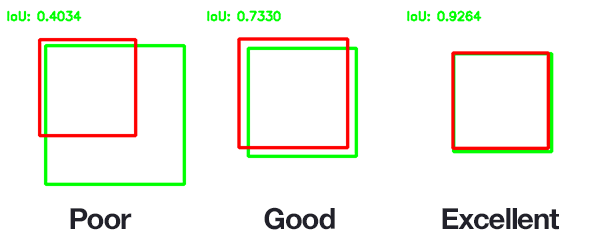
\includegraphics[width=0.95\textwidth]{resources/iou_examples.png}
            \caption{An example of computing Intersection over Unions for various bounding boxes. The predicted bounding boxes are drawn in red color, while the ground-truth ones are drawn in green color. Source: \cite{iourosebrock}.}
            \label{fig:iou-examples}
        \end{figure}
        
    \subsection{\Glsentryfull{mota}}
        The \gls{mota} is most widely used metric for evaluating a tracker's performance. It's main advantage is expressiveness as it combines three different sources of errors.
        
        \begin{itemize}
            \item \textbf{\Gls{fp}} - The number of false positives (incorrect detections).
            \item \textbf{\Gls{fn}} - The number of false negatives (missed detections).
            \item \textbf{\Gls{idsw}} - The number of identity switches.
        \end{itemize}

        The \gls{mota} equation is then given by:
        
        \begin{equation}
            \text{MOTA} = 1 - \frac{\sum_{t} \left( \text{FN}_t + \text{FP}_t + \text{IDSW}_t \right)}{\sum_{t}\text{GT}_t},
        \end{equation}
        
        where $t$ is the frame index and GT is the number of ground-truth objects. The possible values are reported in the percentage from $(-\infty, 100]$. Negative values are possible when the number of errors made exceeds the number of all objects in sequence.
    
    \subsection{\Glsentryfull{motp}} 
        The \gls{motp} represents the average dissimilarity between the ground-truth and the predicted bounding boxes. It is calculated as 
        
        \begin{equation}
            \text{MOTP} = \frac{\sum_{t,i} d_{t,i}}{\sum_{t}c_t},
        \end{equation}
        
        where $c_t$ denotes the number of matches in frame $t$ and $d_t,i$ denotes the bounding box overlap of ground-truth and the predicted target. It thereby gives the average overlap between all correctly matched hypotheses and their respective objects and ranges between $t_d := 50\%$ and $100\%$. \cite{MOTChallenge2015}
    
    \subsection{\Glsentryfull{fps}} 
        The \gls{fps} is common metric used in many fields to measure run-time performance of algorithms, animations, rendering, etc. In this context, it expresses the ability of algorithm to process and analyze a certain number of images per second. With increasing algorithm complexity, the frame rate decreases. Real-time ability in video sequence processing is assumed at 25 \gls{fps} \cite{MOTChallenge2015}.
        
    % \subsection{Mean average precision}
